\subsection{Android Application Package (APK)} \label{subsection:foundation-android-package}
Android applications are installed and distributed in the \gls{apk} file format.
They can either be installed from an appstore like Google Play or downloaded and installed manually or by using \gls{adb} from any other source.
\newline
The \gls{apk} format is based on the ZIP file archive format and contains the resources of the application. The resources are added in the build process which is visualized in figure~\ref{fig:apk}.
\begin{figure}[h]
    \centering
    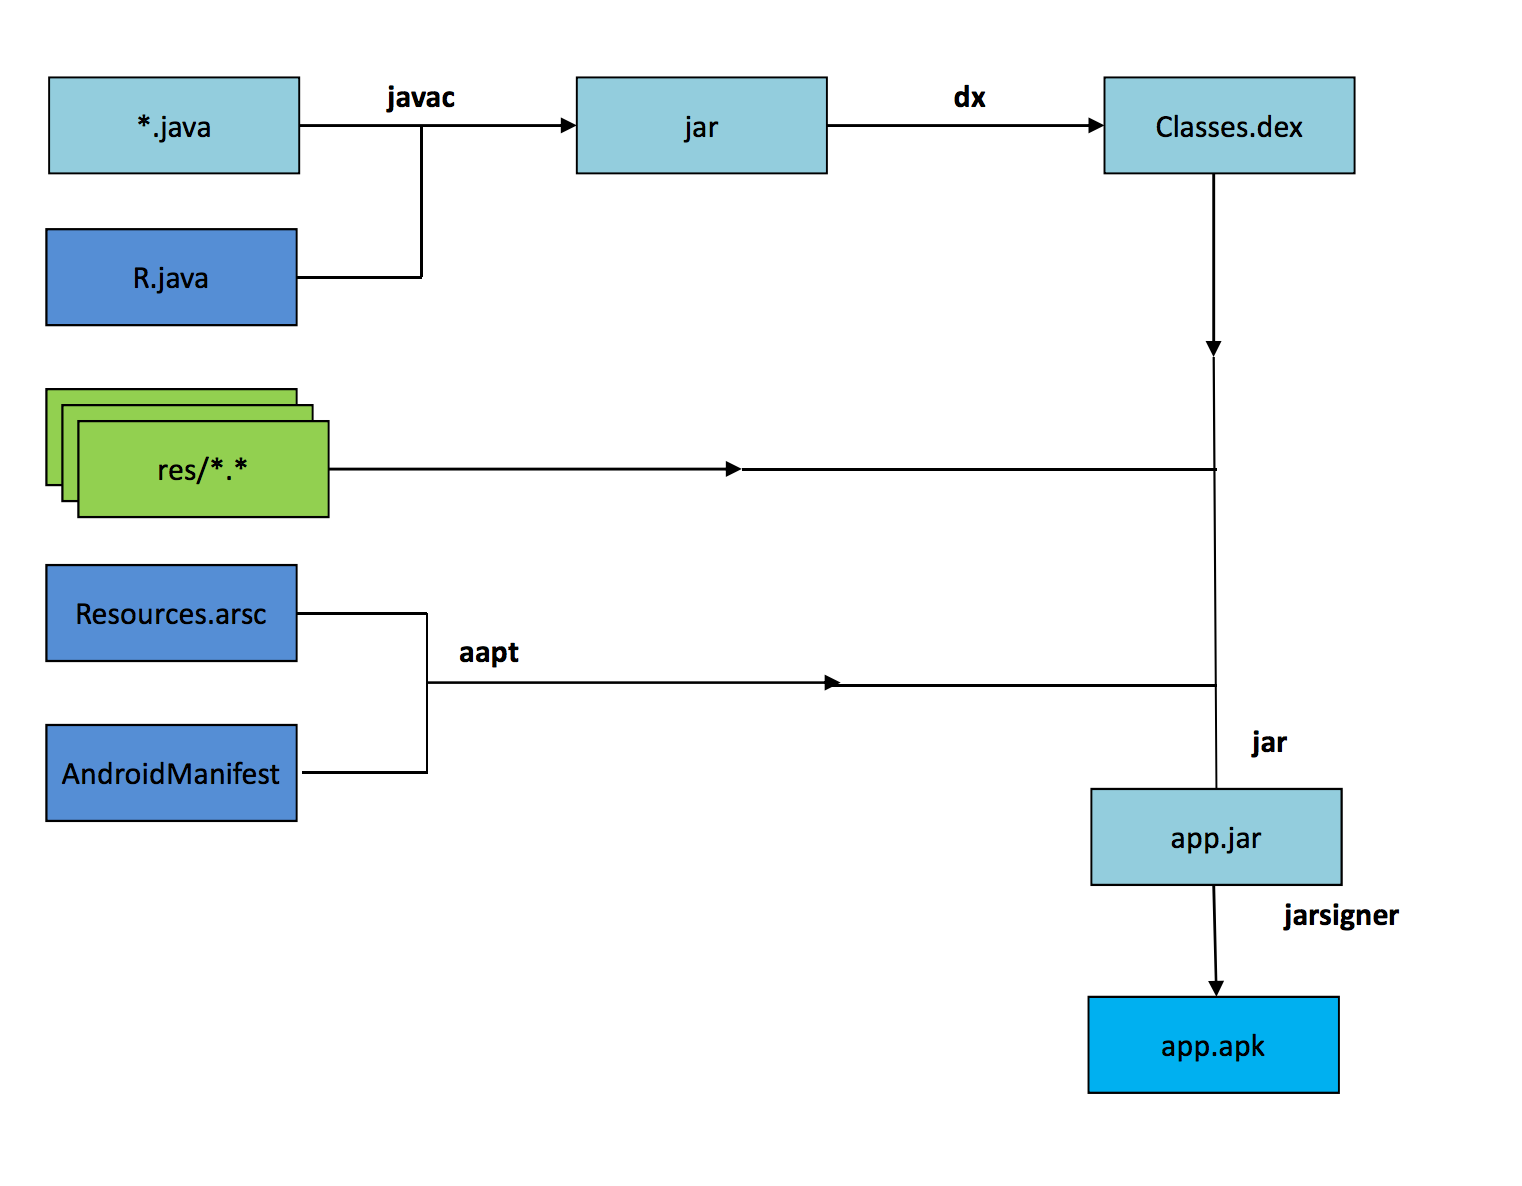
\includegraphics[width=0.8\textwidth]{data/apk.png}
    \caption{apk \cite{andevconDalvikART}}
    \label{fig:apk}
\end{figure}
\newline
Android applications are usually written in Java.

step 1
Java files which will be compiled into \gls{classg} files by a Java Compiler,  similar to a Java program build process, class files contain Java bytecode representing the compiled application, optional step apply a Java Obfuscator\newline
Standard Java environment compiles each separate class in the .java source code file into a corresponding Java bytecode .class file. Each class will be compiled into a single .class file. These are later packed together in a single .jar archive file. The JVM unpacks the .class files, parses and executes their code at runtime.\newline

step 2: transformation from Java bytecode into Dalvik bytecode, see oben, dx programm from android sdk (due to it is necessity for building an application for the Android platform), output saved in singel \gls{dexg} file, included in an APK in next step, possible to apply a further obfuscator operating
on Dalvik bytecode(ERKLÄRUNG)\newline
On the Android platform, the build process differs after the point when the .class files have been generated. Once having the latter, they are forwarded to the “dx” tool which is part of the standard Android SDK. This tool compresses all .class files into a single classes.dex file i.e. the .dex file is the sole bytecode container for all the application’s classes. After it has been created, the classes.dex is forwarded to the ApkBuilder tool altogether with the application resources and shared object (.so) files which, if present, contain native code. As a result, the APK archive is created and the final compulsory step is its signing. Figure 1.2 shows the APK build process and the
possible obfuscation manipulations which are optional during the build stages\newline

In the third step the ApkBuilder creates an \gls{apk} which includes the classes.dex file and other resources.
classes.dex: The classes compiled in the dex file format understandable by the Dalvik virtual machine

In the fourth and final step the jarsigner adds the developers signature to the package.
lib: the directory containing the compiled code that is specific to a software layer of a processor, the directory is split into the different processor types
res: the directory containing resources not compiled into resources.arsc (see below).
assets: a directory containing applications assets, which can be retrieved by AssetManager.
resources.arsc: a file containing precompiled resources, such as binary XML for example.
AndroidManifest.xml: An additional Android manifest file, describing the name, version, access rights, referenced library files for the application. This file may be in Android binary XML that can be converted into human-readable plaintext XML with tools such as AXMLPrinter2, android-apktool, or Androguard.
classes.dex: The classes compiled in the dex file format understandable by the Dalvik virtual machine


The signing does not improve security of the application itself but makes it possible to identify the developer and makes it possible to install updates for the application.
META-INF directory:
    MANIFEST.MF: the Manifest file
    CERT.RSA: The certificate of the application.
    CERT.SF: The list of resources and SHA-1 digest of the corresponding lines in the MANIFEST.MF file



%APK
%The file format of the install ready application is called Android
%Package (APK) and all the mobile software is distributed over Google Play in this format. The APK format is a package management system based on the ZIP file archive format.\newline
%CONTENT:
%META-INF directory:
%    MANIFEST.MF: the Manifest file
%    CERT.RSA: The certificate of the application.
%    CERT.SF: The list of resources and SHA-1 digest of the corresponding lines in the MANIFEST.MF file

%lib: the directory containing the compiled code that is specific to a software layer of a processor, the directory is split into the different processor types

%res: the directory containing resources not compiled into resources.arsc (see below).

%assets: a directory containing applications assets, which can be retrieved by AssetManager.

%AndroidManifest.xml: An additional Android manifest file, describing the name, version, access rights, referenced library files for the application. This file may be in Android binary XML that can be converted into human-readable plaintext XML with tools such as AXMLPrinter2, android-apktool, or Androguard.
%classes.dex: The classes compiled in the dex file format understandable by the Dalvik virtual machine

%resources.arsc: a file containing precompiled resources, such as binary XML for example.

%BUILD PROCESS
%written using the Java programming language.\newline
%Standard Java environment compiles each separate class in the .java source code file into a corresponding Java bytecode .class file. Each class will be compiled into a single .class file. These are later packed together in a single .jar archive file. The JVM unpacks the .class files, parses and executes their code at runtime.\newline
%On the Android platform, the build process differs after the point when the .class files have been generated. Once having the latter, they are forwarded to the “dx” tool which is part of the standard Android SDK. This tool compresses all .class files into a single classes.dex file i.e. the .dex file is the sole bytecode container for all the application’s classes. After it has been created, the classes.dex is forwarded to the ApkBuilder tool altogether with the application resources and shared object (.so) files which, if present, contain native code. As a result, the APK archive is created and the final compulsory step is its signing. Figure 1.2 shows the APK build process and the
%possible obfuscation manipulations which are optional during the build stages\newline


%\cite{kovachevaMaster} \cite{ehringerDalvik}
%


%Aufbau APK erklären\newline

%many steps and tools until the APK is build and ready to be deployed\newline
%applications are written in the Java programming language by the developer, code is available in \gls{classg} files\newline
%step 1:  Java files which will be compiled into \gls{classg} files by a Java Compiler,  similar to a Java program build process, class files contain Java bytecode representing the compiled application, optional step apply a Java Obfuscator\newline
%step 2: transformation from Java bytecode into Dalvik bytecode, see oben, dx programm from android sdk (due to it is necessity for building an application for the Android platform), output saved in singel \gls{dexg} file, included in an APK in next step, possible to apply a further obfuscator operating
%on Dalvik bytecode(ERKLÄRUNG)\newline
%step 3: packing and signing the APK, ApkBuilder constructs an apk file out of the "classes.dex" file and adds further resources like images and ".so" files, ”.so” files are shared objects which contains native functions that can be called from within the DVM, jarsigner adds developers signature to APK(ERKLÄREN WARUM SIGNATURE NÖTIG UND WO GEPRÜFT), now the app can be installed


%It is basically a ZIP-compressed file and contains resources of the application like pictures and layouts as well as a dex file\newline
%This dex file, saved as ”classes.dex”, contains the program code in form of Dalvik bytecode. Further explanations on this bytecode format are given in section 3.2. The content of the APK is also cryptographically signed, which yields no security improvement but helps to distinguish and confirm authenticity of different developers of Android applications.\newline
%DIe apk kann dann per adb, market oder direkt installiert werden\newline
%Within the installation process, every installed application gets its own unique user ID (UID) by default. This means that every application will be executed as a separate system user. -see- QUELLE/SINN?\newline
